\documentclass[12pt]{article}

\usepackage[utf8x]{inputenc}
\usepackage[spanish]{babel}

\usepackage{amssymb,amsmath,amsthm,amsfonts}
\usepackage{calc}
\usepackage{graphicx}
\usepackage{subfigure}
\usepackage{gensymb}
\usepackage{natbib}
\usepackage{url}
\usepackage[utf8x]{inputenc}
\usepackage{amsmath}
\usepackage{graphicx}
\graphicspath{{images/}}
\usepackage{parskip}
\usepackage{fancyhdr}
\usepackage{vmargin}
\setmarginsrb{3 cm}{2.5 cm}{3 cm}{2.5 cm}{1 cm}{1.5 cm}{1 cm}{1.5 cm}

\title{Gitarren Held}					% Titulo
\author{Juan Pablo Abarca T\\
        Nicolás García S\\
        Sebastián Sánchez P}					% Autor
\date{\today}						% Fecha


\makeatletter
\let\thetitle\@title
\let\theauthor\@author
\let\thedate\@date
\makeatother

\pagestyle{fancy}
\fancyhf{}
\rhead{\theauthor}
\lhead{\thetitle}
\cfoot{\thepage}

\begin{document}

%%%%%%%%%%%%%%%%%%%%%%%%%%%%%%%%%%%%%%%%%%%%%%%%%%%%%%%%%%%%%%%%%%%%%%%%%%%%%%%%%%%%%%%%%

\begin{titlepage}
	\centering
    \vspace*{0.0 cm}
    
\includegraphics[scale = 0.5]{ucn.png}\\[1.0 cm]	% Logo Universidad
    
\includegraphics[scale = 2]{logo.png}\\[1.0 cm]	% Logo Universidad
    \textsc{\LARGE Universidad Católica Del Norte}\\[0.5 cm]	% Nombre Universidad		
	\textsc{\large Proyecto de introducción a la ingeniería II}\\[0.5 cm]		% Nombre Curso
	\rule{\linewidth}{0.2 mm} \\[0.4 cm]
	{ \huge \bfseries \thetitle}\\
	\rule{\linewidth}{0.2 mm} \\[1.5 cm]
	
	\begin{minipage}{0.4\textwidth}
		\begin{center} \large
			\emph{Autor:}\\
			\theauthor\linebreak
			\end{center}
	\end{minipage}\\[2 cm]
	
	{\large \thedate}\\[2 cm]
 
	\vfill
	
\end{titlepage}

%%%%%%%%%%%%%%%%%%%%%%%%%%%%%%%%%%%%%%%%%%%%%%%%%%%%%%%%%%%%%%%%%%%%%%%%%%%%%%%%%%%%%%%%%

\tableofcontents
\pagebreak

%%%%%%%%%%%%%%%%%%%%%%%%%%%%%%%%%%%%%%%%%%%%%%%%%%%%%%%%%%%%%%%%%%%%%%%%%%%%%%%%%%%%%%%%%

\section{Introducción}
 \begin{flushleft}
Últimamente el mundo de las enseñanzas de las tecnologías y  la computación, son más estrechas para la sociedad. Uno de los grandes proyectos realizados fue en el año 2003, por los estudiantes del Instituto de Diseño Interactivo de Ivrea, Italia, con el fin de facilitar el acceso y uso de la electrónica y programación. Ellos lo hicieron para que los estudiantes de electrónica tuviesen una alternativa más económica a las populares BASIC Stamp, unas placas que por aquel entonces valían más de cien dólares, y que no todos se podían permitir. 
Es así como nació el proyecto Arduino, que facilita la creación de electrónica de código abierto, la cual está basada en hardware y software libre, flexible y fácil de utilizar para los creadores y desarrolladores.

Diversas son las utilidades que tiene un Arduino en la vida cotidiana, una de ellas es el desarrollo de videojuegos arcade. Debido a esto y al objetivo que presenta el curso Proyecto introducción a la ingeniería II, se desarrollará un mando y el videojuego, el cuál se basará en las bases de “Guitar Hero”.

Cabe destacar que Guitar Hero es una serie de juegos musicales, donde el jugador utiliza un  controlador con características muy similares a una guitarra eléctrica para simular al artista tocando la guitarra, el bajo y en otros casos la banda completa (batería o vacalista). 

Para el desarrollo de este juego, se utilizará el lenguaje de programación Python y Arduino (un lenguaje basado en C++). Además de la aplicación de una librería de Python llamado Pygame, que permiten la creación de videojuegos en dos dimensiones de una manera sencilla. Mediante PyGame se puede utilizar sprites (objetos), cargar y mostrar imágenes en diferentes formatos, sonidos, etc. Tambiém, al ser un módulo destinado a la programación de videojuegos se puede monitorizar el teclado o mando.

La distribución de este informe está estructurado por la historia del videojuego, diseño del mando, descripción de los componentes, descripción del trabajo realizado, problemas encontrados y pruebas realizadas en donde cada uno de ellos está relacionado con el desarrollo del proyecto.
















	\end{flushleft}
	\newpage
	
\section{Historia}
    En el año 2005 las compañías Harmonix y RedOctane lanzaron Guitar Hero para la consola PlayStation 2. A causa del suceso del primer juego de la serie, en el año 2006 fue lanzado Guitar Hero II que fue todo un éxito en el mundo entero. 
    
Al siguiente año RedOctane y Harmonix experimientaron grandes cambios, ya que RedOctane fue comprada por Activision en junio del 2006, en tanto en octubre se anuncia que MTV Networks com paría Harmonix. Trayendo resultados nefastos para la compañía de Harmonix, ya que  no desarrollaría más ningún juego futuro en la serie, pasando la responsabilidad a Neversoft, una subsidiaria de Activision.
Con el lanzamiento de Guitar Hero III: Lengends of Rock, marcó un cambio en la rama de estos videojuegos, ya que fue el primer desarrollo de un guitar hero por la compañía de Neversoft y Activision. 

Con el lanzamiento de Guitar Hero World Tour el juego tuvo un cambio importante en cuanto a géneos musicales, ya que anteriormente Guitar Hero se enfocaba más en el Hard Rock, sin embargo en esta versión los géneros musicales son más variados, por lo que atrajeron a otro público.A partir de entonces, la jugabilidad de la serie Guitar Hero se relacionó con la banda en lugar de solo con la guitarra y el bajo .
Mientras Neversoft trabajaba en los juegos de Guitar Hero para consola, Vicarious Visions trabajó en la serie On Tour, así como en los puertos de Wii de los juegos de Guitar Hero y la versión para iOS de Guitar Hero. Beenox Studios   también trabajó en Guitar Hero: Smash Hits para las consolas.

Aunque Guitar Hero 5 fue lanzado antes de Guitar Hero: Van Halen , Guitar Hero: Van Halen utilizó los elementos de Guitar Hero: Smash Hits y Guitar Hero: Metallica . Neversoft también desarrolló los spin-offs de DJ Hero y Band Hero .

Debido a la falta de juegos de ritmo en las ventas, Guitar Hero: Warriors of Rock fue el último juego de Guitar Hero de Neversoft y sería el último juego de Guitar Hero desarrollado en varios años. Esto se declaró en febrero de 2011.
Sin embargo, Guitar Hero regresó en 2015 con Guitar Hero Live , desarrollado por FreeStyle Games , los desarrolladores de la serie DJ Hero
\newpage
\subsection{Títulos de Guitar Hero en la historia}
    \begin{itemize}
        \item Guitar Hero (2005)
        \item Guitar Hero II (2006)
        \item Guitar Hero III: Legends of Rock (2007)
        \item 	Guitar Hero World Tour (2008)
         \item Guitar Hero 5 (2009)
        \item 	Guitar Hero: Guerreros del Rock (2010)
        \item Guitar Hero Live (2015)
        \newline
    \end{itemize}
    \subsection{Juegos spin-off}
    \begin{itemize}
        \item Guitar Hero Encore: Rocks the 80s (2007)
        \item Guitar Hero: Smash Hits (2009)
        \item	Band Hero (2009)
        \newline
    \end{itemize}
    \subsection{Spin-offs relacionados con la banda}
    \begin{itemize}
      \item Guitar Hero: Aerosmith (2008)
      \item Guitar Hero: Metallica (2009)
      \item Guitar Hero: Van Halen (2009)
    \newline
    \end{itemize}
    \subsection{En la serie Tour}
    \begin{itemize}
     \item	Guitar Hero: de gira (2008)
     \item	Guitar Hero: décadas (2008)
    \item Guitar Hero On Tour: Modern Hits (2009)


    \end{itemize}
    
    
    
  
\newpage
\section{Diseño del mando}
    El mando estara formado por:
    \begin{itemize}
        \item \textbf{Botonera:}
        Esta compuesta por 5 botones de distintos colores : Verde,Rojo ,Azul ,Amarillo , Naranjo.
        \item \textbf{Star/Select:}
        Esta compuesto por el boton Start y select en la parte posterior de la Guitarra
         \item \textbf{Slayer:}
         Ubicado en la parte central de la Guitarra
    \end{itemize}

    
    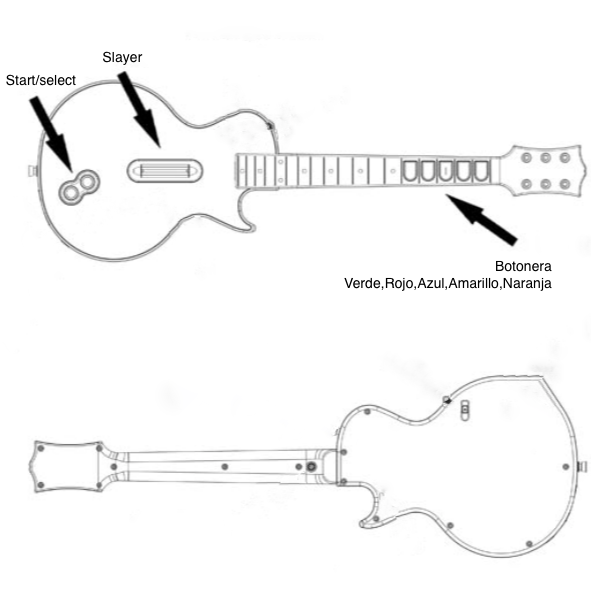
\includegraphics[scale = 0.5]{diseno.png}\\[1.0 cm]
    \newpage
\section{Descripción de componentes}
    \subsection{Arduino Due }
    \begin{itemize}
        \item \textbf{Función y para que sirve }: Arduino es una plataforma de hardware libre, basada en una placa con un microcontrolador y un entorno de desarrollo (software), diseñada para facilitar el uso de la electrónica en proyectos multidisciplinares. Arduino es utilizado para tomar información del entorno a través de sus pines de entrada de toda una gama de sensores y puede afectar aquello que le rodea controlando luces, motores y otros componentes.
        \item \textbf{Pines utilizados }: Para este proyecto los pines que se utilizarán de la categoría Digital (PWM) son : \textbf{GND,22, 23, 24, 25, 26, 27, 28 y 29.} Y en categoría Power:\textbf{ 3.3 v.}
        \item\textbf{Ejemplo de uso en otros ámbitos: }Un Arduino puede ser utilizado en muchos proyectos de diversas temáticas, por ejemplo crear un termómetro arduino para medir la temperatura ambiental. Otro uso que se puede aplicar, es la automatización de sistemas ( sistema de regadío).
        \newline
        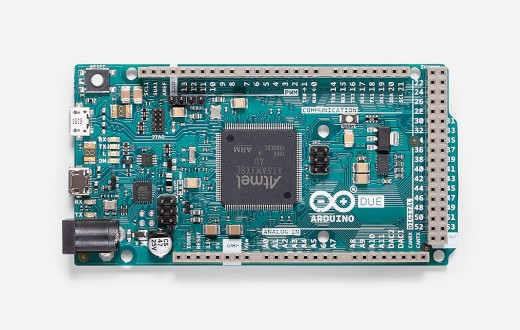
\includegraphics[scale = 1]{due.png}\\[1.0 cm]
    \end{itemize}{}
    \subsection{Interruptor final de carrera}
    \begin{itemize}
         \item \textbf{Función y para que sirve: }Interruptor de final de carrera son dispositivos electromecánicos que constan de un accionador vinculado mecánicamente a un conjunto de contactos. Cuando un objeto entra en contacto con el accionador, el dispositivo opera los contactos para cerrar o abrir una conexión eléctrica.
         \item \textbf{Pines utilizados: }1 COM y 3NO.
         \item\textbf{Ejemplo de uso en otros ámbitos: }Son muy habituales en la industria para detectar la llegada de un elemento móvil a una determinada posición.
        \newline
        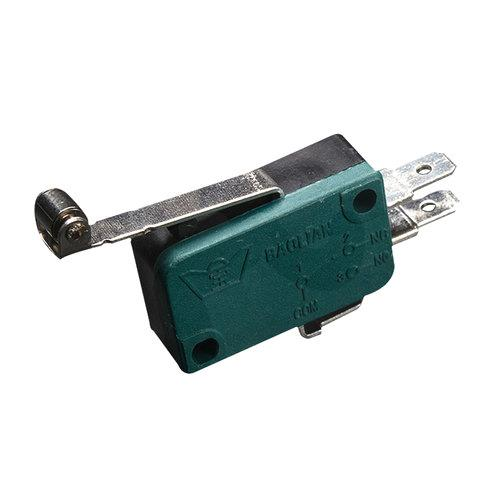
\includegraphics[scale =0.7]{finaldecarrera.png}\\[1.0 cm]
    \end{itemize}{}
    \subsection{Pulsador switch de 12mm.}
    \begin{itemize}
         \item \textbf{Función y para que sirve }:Un pulsador es un operador eléctrico que, cuando se oprime, permite el paso de la corriente eléctrica y, cuando se deja de oprimir, lo interrumpe.
         \item \textbf{Pines utilizados: }4 pines.
         \item\textbf{Ejemplo de uso en otros ámbitos: }Son muy habituales en la industria para detectar la llegada de un elemento móvil a una determinada posición.
         \newline
         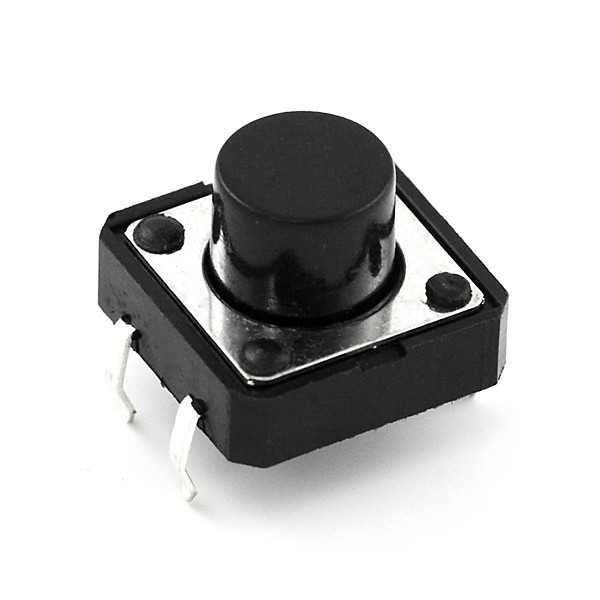
\includegraphics[scale =0.3]{switch.png}\\[1.0 cm]
    \end{itemize}{}
        \newpage
         \subsection{Diagrama de conexión Elèctrica:}
         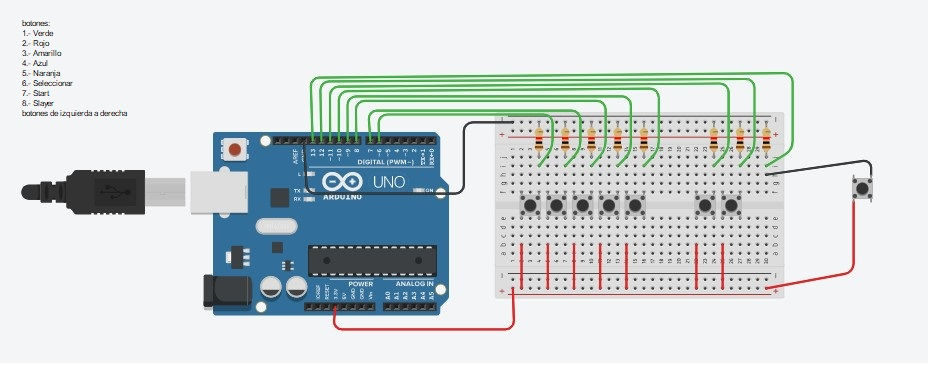
\includegraphics[scale =0.7]{diagrama.png}\\[0.2 cm]
         \newpage
\section{Trabajo realizado}
    Una vez que se informó el juego a realizar y ver en que consistía se investigo el control ideal para este proyecto, con lo cual salió que un estilo guitarra era la mejor idea de dar la comodidad necesaria y jugabilidad.
    
Se empezó a desarrollar un bosquejo en el cual debíamos integrar el Arduino y una protoboard, para poder conectar los distintos switch, a continuación, se desarrollaron clases en las cuales nos dieron información de como programar un Arduino y se hicieron distintas pruebas con botones y luces led 
Luego se decidió el empezar a desarrollar el código para la funcionalidad del Arduino con los botones, todo esto se hacia suponiendo ya que no habían llegado los materiales, por lo que se procedió a desarrollar en el programa “Fusion-360” el control o piezas para este. se hicieron bosquejos los cuales se enviaron para poder realizar la impresión 3d. 

En la 6° semana llegaron los componentes para poder realizar la configuración del control con lo cual se puso a trabajar, conectar para probar codificación realizada y ver el correcto funcionamiento de todo el sistema, en eso ya probado todo el funcionamiento sin errores, se enlazo el Arduino a Phyton para ver que la configuración sea la correcta y este lo leyera.
    \newpage

\section{Problemas surgidos}
    Uno de los principales problemas que se presento fue la intermitencia de datos al momento de interpretarlos , mediante “Monitor de serie” proporcionado por el IDE de Arduino.
    
Al momento de monitorear estos datos se generaba una intermitencia entre los valores “0” y “1”.
El valor esperado a recibir es un arreglo de enteros [0,0,0,0,0,0,0,0] donde “0” representa “Released” y “1” “Pressed”.


 Por lo mencionado anteriormente,al momento de mantener pulsado un boton el\textbf{    resultado obetenido fue :}
 
[1,0,0,0,0,0,0,0],[0,0,0,0,0,0,0,0],[1,0,0,0,0,0,0,0],[0,0,0,0,0,0,0,0]….

\textbf{Cuando el resultado esperado se representa por:}

[1,0,0,0,0,0,0,0],[1,0,0,0,0,0,0,0],[1,0,0,0,0,0,0,0],[1,0,0,0,0,0,0,0]….


La solución de este fallo se encontraba en el uso de resistencias,si bien estas forman parte del sistema de hardware desde el comienzo,no contaban con la ubicación correctar,por lo tanto no existe un control de voltaje ,provocando la intermitencia de datos.

\section{Pruebas realizadas}
    Las primeras pruebas realizadas en este proyecto se pueden apreciar con mayor detalle en la tabla que se presenta a continuación. A grandes rasgos podemos diferenciar las pruebas por el monitor serial que presenta el entorno de desarrollo de Arduino. Que es el cable entre el ordenador y el Arduino DUE, y así permite enviar y recibir mensajes de texto, útiles para la depuración y también control de Arduino. 
    
    \begin{table}[htbp]
    \begin{center}
    \begin{tabular}{|1|1|1|}
    \hline  
    Botones & Pin & MonitorSerial \\
    \hline 
    Verde & 22 & [1,0,0,0,0,0,0,0] \\ \hline
    Rojo & 23 & [0,1,0,0,0,0,0,0] \\ \hline
    Azul & 24 & [0,0,1,0,0,0,0,0] \\ \hline
    Amarillo & 25 & [0,0,0,1,0,0,0,0] \\ \hline
    Naranja & 26 & [0,0,0,0,1,0,0,0] \\ \hline
    Start & 27 & [0,0,0,0,0,1,0,0] \\ \hline
    Select & 22 & [0,0,0,0,0,0,1,0] \\ \hline
    Slayer & 22 & [0,0,0,0,0,0,0,1] \\ \hline
    \end{tabular}
    \caption{Tabla Monitor de Serie Arduino.}
    \label{tabla:sencilla}
    \end{center}
    \end{table}
    
    
    
\section{Conclusión}

Arduino es una nueva forma de enseñanza del hardware y software de la computación básica, el cual permite ampliar la mirada del nuevo desarrollador, generando mayores competencias para aplicarlo en su vida cotidiana.Para disminuir estas brechas de conocimiento, el curso de “Introducción a la ingeniería II” permitió el complemento entre el desarrollo de un videojuego y la fabricación de un mando.

 Como grupo de trabajo se concluyó que Arduino es un lenguaje de programación sencillo de combinar con algún indicador o un testigo (consola de pruebas) para poder hacer la compilación con el videojuego.Además de tener los conocimientos fundamentales de electrónica y de programación, para generar el control del videojuego.
 
Otro punto a destacar es la gran posibilidad de manejar un ámbito mas general en el desarrollo de software, aplicaciones y juegos.

La primera etapa de este proyecto termina con el desarrollo del control, hasta obtener un protoboard conectado con 7 botones y 1 Interruptor final de carrera, además de las resistencias y cables, todas ellas unidas al Arduino DUE y así tener las bases para continuar con el desarrollo del videojuego.

\newpage
\section{ Referencias}
    \begin{itemize}
    \item Qué es Arduino, cómo funciona y qué puedes hacer con uno. (2018).
    Recuperado el 06 de octubre de 2019, de https://www.xataka.com/basics/que-arduino-como-funciona-que-puedes-hacer-uno. 
    
    \item Programación con Arduino, el paradigma de la computación física. (2017). 
    Recuperado el 06 de octubre de 2019, de https://programarfacil.com/podcast/programar-arduino-la-computacion-fisica/.
    
     \item Aprendiendo Arduino. (2016).
     
     Recuperado el 06 de octubre de 2019,
     
     de https://aprendiendoarduino.wordpress.com/category/monitor-serie/.
     
     \item Tecnología de los pulsadores e interruptores (2006). Recuperado el 06 de octubre de 2019, de https://www.abc.com.py/edicion-impresa/suplementos/escolar/tecnologia-de-los-pulsadores-e-interruptores-904222.html.
     
    \item ¿Qué son los interruptores finales de carrera? (2009). 
    Recuperado el 06 de octubre de 2019, de https://www.quiminet.com/articulos/que-son-los-interruptores-finales-de-carrera-7838.html
    
    \item Tipos de arduino y sus funciones (2012). Recuperado el 06 de octubre de 2019, de http://danimtzc.blogspot.com/2012/05/tipos-de-arduino-y-sus-funciones.html?m=1
    
    \end{itemize}

\end{document}